% FID values for run8 and run9
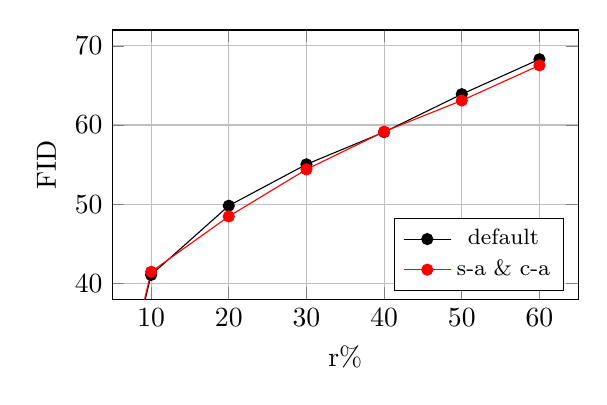
\begin{tikzpicture}
\begin{axis}[
    title={},
    height=5cm,
    width=7.5cm,
    xlabel={r\%},
    ylabel={FID},
    xmin=5, xmax=65,
    ymin=38, ymax=72,
    xtick={10,20,30,40,50,60},
    ytick={30,40,50,60,70},
    legend pos=south east,
    xmajorgrids=true,
    ymajorgrids=true,
    legend style={font=\footnotesize}
]

\addplot[
    color=black,
    mark=*
    ]
    coordinates {
    (0,0)(10,41.06)(20,49.80)(30,55.03)(40,59.10)(50,63.89)(60,68.30)
    };
    
\addplot[
    color=red,
    mark=*
    ]
    coordinates {
    (0,0)(10,41.45)(20,48.45)(30,54.39)(40,59.16)(50,63.09)(60,67.53)
    };
    
\legend{default, s-a \& c-a}
    
\end{axis}
\end{tikzpicture}